% Options for packages loaded elsewhere
\PassOptionsToPackage{unicode}{hyperref}
\PassOptionsToPackage{hyphens}{url}
%
\documentclass[
  ignorenonframetext,
]{beamer}
\usepackage{pgfpages}
\setbeamertemplate{caption}[numbered]
\setbeamertemplate{caption label separator}{: }
\setbeamercolor{caption name}{fg=normal text.fg}
\beamertemplatenavigationsymbolsempty
% Prevent slide breaks in the middle of a paragraph
\widowpenalties 1 10000
\raggedbottom
\setbeamertemplate{part page}{
  \centering
  \begin{beamercolorbox}[sep=16pt,center]{part title}
    \usebeamerfont{part title}\insertpart\par
  \end{beamercolorbox}
}
\setbeamertemplate{section page}{
  \centering
  \begin{beamercolorbox}[sep=12pt,center]{part title}
    \usebeamerfont{section title}\insertsection\par
  \end{beamercolorbox}
}
\setbeamertemplate{subsection page}{
  \centering
  \begin{beamercolorbox}[sep=8pt,center]{part title}
    \usebeamerfont{subsection title}\insertsubsection\par
  \end{beamercolorbox}
}
\AtBeginPart{
  \frame{\partpage}
}
\AtBeginSection{
  \ifbibliography
  \else
    \frame{\sectionpage}
  \fi
}
\AtBeginSubsection{
  \frame{\subsectionpage}
}
\usepackage{lmodern}
\usepackage{amssymb,amsmath}
\usepackage{ifxetex,ifluatex}
\ifnum 0\ifxetex 1\fi\ifluatex 1\fi=0 % if pdftex
  \usepackage[T1]{fontenc}
  \usepackage[utf8]{inputenc}
  \usepackage{textcomp} % provide euro and other symbols
\else % if luatex or xetex
  \usepackage{unicode-math}
  \defaultfontfeatures{Scale=MatchLowercase}
  \defaultfontfeatures[\rmfamily]{Ligatures=TeX,Scale=1}
\fi
% Use upquote if available, for straight quotes in verbatim environments
\IfFileExists{upquote.sty}{\usepackage{upquote}}{}
\IfFileExists{microtype.sty}{% use microtype if available
  \usepackage[]{microtype}
  \UseMicrotypeSet[protrusion]{basicmath} % disable protrusion for tt fonts
}{}
\makeatletter
\@ifundefined{KOMAClassName}{% if non-KOMA class
  \IfFileExists{parskip.sty}{%
    \usepackage{parskip}
  }{% else
    \setlength{\parindent}{0pt}
    \setlength{\parskip}{6pt plus 2pt minus 1pt}}
}{% if KOMA class
  \KOMAoptions{parskip=half}}
\makeatother
\usepackage{xcolor}
\IfFileExists{xurl.sty}{\usepackage{xurl}}{} % add URL line breaks if available
\IfFileExists{bookmark.sty}{\usepackage{bookmark}}{\usepackage{hyperref}}
\hypersetup{
  pdftitle={MA8701 Advanced methods in statistical inference and learning},
  pdfauthor={Mette Langaas IMF/NTNU},
  hidelinks,
  pdfcreator={LaTeX via pandoc}}
\urlstyle{same} % disable monospaced font for URLs
\newif\ifbibliography
\usepackage{color}
\usepackage{fancyvrb}
\newcommand{\VerbBar}{|}
\newcommand{\VERB}{\Verb[commandchars=\\\{\}]}
\DefineVerbatimEnvironment{Highlighting}{Verbatim}{commandchars=\\\{\}}
% Add ',fontsize=\small' for more characters per line
\usepackage{framed}
\definecolor{shadecolor}{RGB}{248,248,248}
\newenvironment{Shaded}{\begin{snugshade}}{\end{snugshade}}
\newcommand{\AlertTok}[1]{\textcolor[rgb]{0.94,0.16,0.16}{#1}}
\newcommand{\AnnotationTok}[1]{\textcolor[rgb]{0.56,0.35,0.01}{\textbf{\textit{#1}}}}
\newcommand{\AttributeTok}[1]{\textcolor[rgb]{0.77,0.63,0.00}{#1}}
\newcommand{\BaseNTok}[1]{\textcolor[rgb]{0.00,0.00,0.81}{#1}}
\newcommand{\BuiltInTok}[1]{#1}
\newcommand{\CharTok}[1]{\textcolor[rgb]{0.31,0.60,0.02}{#1}}
\newcommand{\CommentTok}[1]{\textcolor[rgb]{0.56,0.35,0.01}{\textit{#1}}}
\newcommand{\CommentVarTok}[1]{\textcolor[rgb]{0.56,0.35,0.01}{\textbf{\textit{#1}}}}
\newcommand{\ConstantTok}[1]{\textcolor[rgb]{0.00,0.00,0.00}{#1}}
\newcommand{\ControlFlowTok}[1]{\textcolor[rgb]{0.13,0.29,0.53}{\textbf{#1}}}
\newcommand{\DataTypeTok}[1]{\textcolor[rgb]{0.13,0.29,0.53}{#1}}
\newcommand{\DecValTok}[1]{\textcolor[rgb]{0.00,0.00,0.81}{#1}}
\newcommand{\DocumentationTok}[1]{\textcolor[rgb]{0.56,0.35,0.01}{\textbf{\textit{#1}}}}
\newcommand{\ErrorTok}[1]{\textcolor[rgb]{0.64,0.00,0.00}{\textbf{#1}}}
\newcommand{\ExtensionTok}[1]{#1}
\newcommand{\FloatTok}[1]{\textcolor[rgb]{0.00,0.00,0.81}{#1}}
\newcommand{\FunctionTok}[1]{\textcolor[rgb]{0.00,0.00,0.00}{#1}}
\newcommand{\ImportTok}[1]{#1}
\newcommand{\InformationTok}[1]{\textcolor[rgb]{0.56,0.35,0.01}{\textbf{\textit{#1}}}}
\newcommand{\KeywordTok}[1]{\textcolor[rgb]{0.13,0.29,0.53}{\textbf{#1}}}
\newcommand{\NormalTok}[1]{#1}
\newcommand{\OperatorTok}[1]{\textcolor[rgb]{0.81,0.36,0.00}{\textbf{#1}}}
\newcommand{\OtherTok}[1]{\textcolor[rgb]{0.56,0.35,0.01}{#1}}
\newcommand{\PreprocessorTok}[1]{\textcolor[rgb]{0.56,0.35,0.01}{\textit{#1}}}
\newcommand{\RegionMarkerTok}[1]{#1}
\newcommand{\SpecialCharTok}[1]{\textcolor[rgb]{0.00,0.00,0.00}{#1}}
\newcommand{\SpecialStringTok}[1]{\textcolor[rgb]{0.31,0.60,0.02}{#1}}
\newcommand{\StringTok}[1]{\textcolor[rgb]{0.31,0.60,0.02}{#1}}
\newcommand{\VariableTok}[1]{\textcolor[rgb]{0.00,0.00,0.00}{#1}}
\newcommand{\VerbatimStringTok}[1]{\textcolor[rgb]{0.31,0.60,0.02}{#1}}
\newcommand{\WarningTok}[1]{\textcolor[rgb]{0.56,0.35,0.01}{\textbf{\textit{#1}}}}
\usepackage{graphicx,grffile}
\makeatletter
\def\maxwidth{\ifdim\Gin@nat@width>\linewidth\linewidth\else\Gin@nat@width\fi}
\def\maxheight{\ifdim\Gin@nat@height>\textheight\textheight\else\Gin@nat@height\fi}
\makeatother
% Scale images if necessary, so that they will not overflow the page
% margins by default, and it is still possible to overwrite the defaults
% using explicit options in \includegraphics[width, height, ...]{}
\setkeys{Gin}{width=\maxwidth,height=\maxheight,keepaspectratio}
% Set default figure placement to htbp
\makeatletter
\def\fps@figure{htbp}
\makeatother
\setlength{\emergencystretch}{3em} % prevent overfull lines
\providecommand{\tightlist}{%
  \setlength{\itemsep}{0pt}\setlength{\parskip}{0pt}}
\setcounter{secnumdepth}{-\maxdimen} % remove section numbering

\title{MA8701 Advanced methods in statistical inference and learning}
\subtitle{L1: Introduction}
\author{Mette Langaas IMF/NTNU}
\date{09 January, 2021}

\begin{document}
\frame{\titlepage}

\begin{frame}

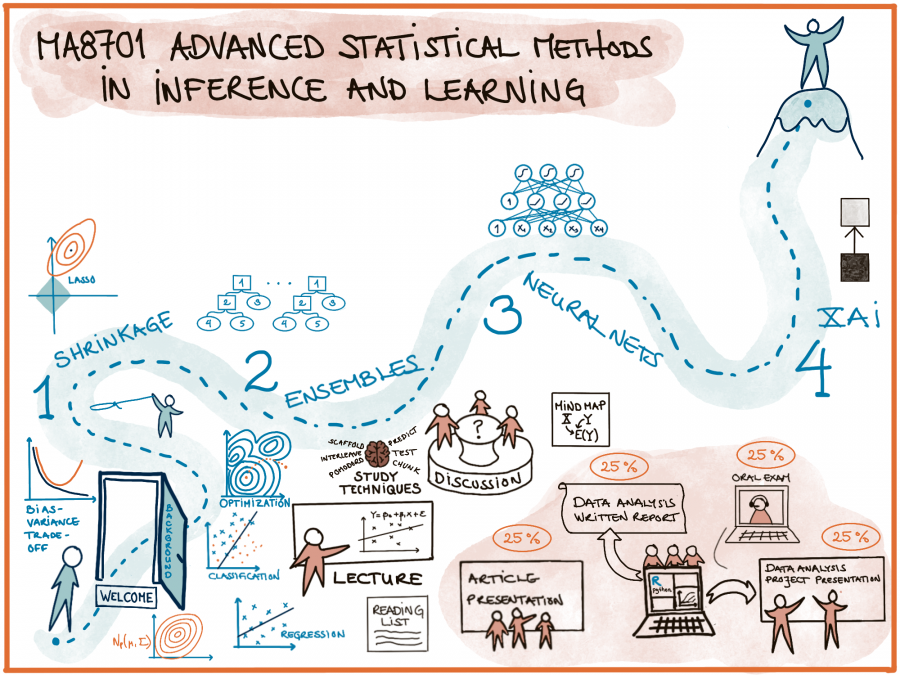
\includegraphics{./overviewv1.png}

\end{frame}

\begin{frame}{Course topics}
\protect\hypertarget{course-topics}{}

\begin{flushleft}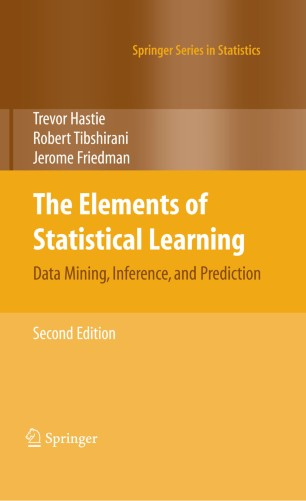
\includegraphics[width=0.2\linewidth]{ELSbookcover} \end{flushleft}

The starting point is that we cover important parts of

The Elements of Statistical Learning: Data Mining, Inference, and
Prediction, Second Edition (Springer Series in Statistics, 2009) by
Trevor Hastie, Robert Tibshirani, and Jerome Friedman.

but, since the book is from 2008 this means that for many topic we need
(to be up to date) additional selected material in the form of book
chapters and research articles.

\end{frame}

\begin{frame}

\begin{block}{Introduction {[}this part, one week{]}}

Sort out assumed background knowledge, and learn something new

\begin{itemize}
\tightlist
\item
  Notation
\item
  Statistical decision theoretic framework (partly new)
\item
  Regression (what do we know)
\item
  Classification (ditto)
\item
  Model selection and model assessment - including bias-variance
  trade-off (mostly new)
\end{itemize}

\end{block}

\end{frame}

\begin{frame}

\begin{block}{Part 1: Shrinkage {[}3 weeks{]}}

or ``Regularized linear and generalized linear models''.

\begin{itemize}
\tightlist
\item
  ELS 3.2.3,3.4, 3.8, 4.4.4.
\item
  Hastie, Tibshirani, Wainwright (HTW): ``Statistical Learning with
  Sparsity: The Lasso and Generalizations''. Selected chapters.
\item
  Post-selective inference (articles)
\item
  An introduction to analysing text
\end{itemize}

Includes one data analysis project with short report.

\end{block}

\end{frame}

\begin{frame}

\begin{block}{Part 2: Ensembles {[}4 (5) weeks{]}}

\begin{itemize}
\tightlist
\item
  trees, bagging and forests
\item
  general ensembles (similar to super learner)
\item
  boosting
\item
  hyper-parameter tuning
\end{itemize}

Selected chapters in ELS (8.7, 8.8, 9.2, parts of 10, 15, 16) and
several articles.

\end{block}

\begin{block}{Part 3: Neural nets {[}(2) 3 weeks{]}}

\begin{itemize}
\tightlist
\item
  Goodfellow, Bengio, Courville: Deep learning (2016). MIT press.
  \url{https://www.deeplearningbook.org/}. Selected chapters.
\item
  Evaluating uncertainty
\end{itemize}

\end{block}

\end{frame}

\begin{frame}

\begin{block}{Part 4: XAI {[}2 weeks{]}}

Lectured by Kjersti Aas \url{https://www.nr.no/~kjersti/}.

Articles on

\begin{itemize}
\tightlist
\item
  LIME,
\item
  partial dependence plots,
\item
  Shapley values,
\item
  relative weights and
\item
  counterfactuals.
\end{itemize}

\end{block}

\begin{block}{Closing {[}1 week{]}}

\begin{itemize}
\tightlist
\item
  w/oral presentations of second data project from Parts 2-4.
\end{itemize}

\end{block}

\end{frame}

\begin{frame}

\begin{block}{Required previous knowledge}

\begin{itemize}
\tightlist
\item
  TMA4267 Linear statistical methods
\item
  TMA4268 Statistical learning
\item
  TMA4295 Statistical inference
\item
  TMA4300 Computer intensive statistical methods
\item
  TMA4315 Generalized linear models
\item
  Good understanding and experience with R, or with Python, for
  statistical data analysis.
\item
  Knowledge of RMarkdown for writing reports and presentations
\item
  Skills in group work - possibly using git
\end{itemize}

\end{block}

\end{frame}

\begin{frame}{Learning}
\protect\hypertarget{learning}{}

\begin{block}{Learning outcome}

\textbf{1. Knowledge}

\begin{itemize}
\tightlist
\item
  Understand and explain the central theoretical aspects in statistical
  inference and learning.
\item
  Understand and explain how to use methods from statistical inference
  and learning to perform a sound data analysis.
\item
  Be able to evaluate strengths and weaknesses for the methods and
  choose between different methods in a given data analysis situation.
\end{itemize}

\end{block}

\end{frame}

\begin{frame}

\textbf{2. Skills}

Be able to analyse a dataset using methods from statistical inference
and learning in practice (using R or Python), and give a good
presentation and discussion of the choices done and the results found.

\textbf{3. Competence}

\begin{itemize}
\tightlist
\item
  The students will be able to participate in scientific discussions,
  read research presented in statistical journals, and carry out
  research in statistics at high international level.
\item
  They will be able to participate in applied projects, and analyse data
  using methods from statistical inference and learning.
\end{itemize}

\end{frame}

\begin{frame}

\begin{block}{Learning methods and activities}

Herbert A. Simon (Cognitive science, Nobel Laureate): \emph{Learning
results from what the student does and thinks and only from what the
student does and thinks. The teacher can advance learning only by
influencing what the student does to learn.}

\begin{itemize}
\item
  Lectures will be on 14 Mondays 9.15-12 in S21 (and zoom). We will not
  record the lectures because we will try to include student activities
  in groups (on tables or break-out rooms).
\item
  Exploring different study techniques (one or more each lecture).
\item
  Problem sets to work on between lectures.
\item
  Final individual oral exam (25\% of pass/fail grade) in May.
\end{itemize}

\end{block}

\end{frame}

\begin{frame}

\begin{itemize}
\item
  One practical compulsory group project in data analysis (application
  of course theory using R or Python) with short report. Topic: Part 1
  on Shrinkage, chosen data set discussed with lecturer before start.
  Due mid February. First given comments by one other group, then
  evaluated by course responsible. (25\% of pass/fail grade)
\item
  One article group presentation, orally (15 minutes+questions).
  Material from Parts 2 and 3 preferred, and must be decided on with
  lecturer (might also be parts of your own master thesis if
  applicable). Due before Easter. (25\% of pass/fail)
\item
  Practical compulsory project in data analysis (application of course
  theory using R or Python) with oral presentation (15
  minutes+questions). Topic: Part 2-4, data set and methods discussed
  with lecturer before start. Due after Part 4 is finished. (25\% of
  pass/fail grade)
\item
  For the two data analysis projects: one should be with a data set
  requiring regression and one with classification type analysis.
\end{itemize}

\end{frame}

\begin{frame}

\begin{block}{Course wiki}

\url{https://wiki.math.ntnu.no/ma8701/2021v/start}

\textbf{Questions?}

\end{block}

\end{frame}

\begin{frame}[fragile]

\begin{block}{Class activity}

Aim: get to know each other - to improve on subsequent group work!

\begin{Shaded}
\begin{Highlighting}[]
\ControlFlowTok{while}\NormalTok{ (at least one student not presented) }
\NormalTok{   lecturer give two alternatives, you choose one. }
\NormalTok{   lecturer choose a few students to present their view }
\NormalTok{   together with giving their name and study programme }
\NormalTok{   (and say }\ControlFlowTok{if}\NormalTok{ they are looking }\ControlFlowTok{for}\NormalTok{ group members)}
\end{Highlighting}
\end{Shaded}

\end{block}

\end{frame}

\begin{frame}

\begin{itemize}
\tightlist
\item
  Dog person or cat person?
\item
  When performing logistic regression - do you then say you do
  statistical learning or machine learning?
\item
  I will show you the result of a descriptive analysis: summary or
  graphical display?
\item
  Learning something new: read a book or watch a video?
\item
  Analysing data: R or python?
\item
  Analysing data: report p-values and or confidence intervals
\item
  In class: taking notes or not?
\item
  Use camel case or snake case for programming?
\end{itemize}

camel: writing compound words such that each word in the middle of the
phrase begins with a capital letter, with no intervening spaces or
punctuation. ``camelCase'' or ``CamelCase''.

snake: writing compound words where the elements are separated with one
underscore character (\_) and no spaces, with each element's initial
letter usually lower cased within the compound and the first letter
either upper- or lower case as in ``foo\_bar''

\end{frame}

\begin{frame}{Introduction}
\protect\hypertarget{introduction}{}

(finally - we start on the fun stuff!)

\begin{block}{Plan}

\begin{itemize}
\tightlist
\item
  Notation
\item
  Statistical decision theoretic framework (partly new)
\end{itemize}

Remind about assumed background knowledge (already known),

\begin{itemize}
\tightlist
\item
  Regression (ELS ch 3, except 3.2.3, 3.2.4, 3.4, 3.7, 3.8)
\item
  Classification (ELS ch 4.1-4.5, except 4.4.4)
\end{itemize}

and then cover new aspects for

\begin{itemize}
\tightlist
\item
  Model selection and assessment (ELS Ch 7.1-7.6, 7.10-7.12), including
  statistical learning and the bias-variance trade-off (ELS ch 2)
\end{itemize}

\end{block}

\end{frame}

\begin{frame}

\begin{block}{Notation}

(mainly from ELS)

We will only consider supervised methods.

\begin{itemize}
\tightlist
\item
  Response \(Y\) (or \(G\)): dependent variable, outcome, usually
  univariate (but may be multivariate)

  \begin{itemize}
  \tightlist
  \item
    quantitative \(Y\): for regression
  \item
    qualitative, categorical \(G\): for classification, some times dummy
    variable coding used (named one-hot coding in machine learning)
  \end{itemize}
\item
  Covariates \(X_1, X_2, \ldots, X_p\): ``independent variables'',
  predictors, features

  \begin{itemize}
  \tightlist
  \item
    continuous, discrete: used directly
  \item
    categorical, discrete: often dummy variable coding used
  \end{itemize}
\end{itemize}

We aim to construct a rule, function, learner: \(f(X)\), to predict
\(Y\) (or \(G\)).

\end{block}

\end{frame}

\begin{frame}

Random variables and (column) vectors are written as uppercase letters
\(X\), and \(Y\), while observed values are written with lowercase
\((x,y)\). (Dimensions specified if needed.)

Matrices are presented with bold face: \({\bf X}\), often
\(N \times (p+1)\).

ELS uses boldface also for \({\bf x}_j\) being a vector of all \(N\)
observations of variable \(j\), but the vector of observed variables for
observation \(i\) is just \(x_i\).

\end{frame}

\begin{frame}

Both the response \emph{and covariates} will be considered to be random,
and drawn from some joint distribution
\(P(X_1,X_2,\ldots, X_p,Y)=P(X,Y)\) or \(P(X,G)\).

Conditional distribution: \(P(X,Y)=P(Y \mid X)P(X)\) or
\(P(Y\mid X=x)P(X=x)\)

and double expectation is often used

\[\text{E}[L(Y,f(X))]=\text{E}_{X,Y}[L(Y,f(X))]=\text{E}_{X}\text{E}_{Y \mid X}[L(Y,f(X))]\]
where \(L\) is a loss function (to be defined next) and \(f(X)\) some
function to predict \(Y\) (or \(G\)).

\end{frame}

\begin{frame}

\begin{block}{Training set}

(ELS 2.1)

A set of size \(N\) of independent pairs \((x_i,y_i)\) is called the
\emph{training set} and often denoted \({\cal T}\).

The training data is used to estimate the unknown function \(f\).

Test data is in general thought of as future data, and plays an
important role in both

\begin{itemize}
\tightlist
\item
  model selection (finding the best model among a candidate set) and
  also for
\item
  model assessment (assess the performance of the fitted model on future
  data).
\end{itemize}

We will consider theoretical results for future test data, and also look
at different ways to split or resample available data.

\end{block}

\end{frame}

\begin{frame}

\begin{block}{Group discussion}

Two core regression methods are multiple linear regression (MLR) and
\(k\)-nearest neighbour (kNN).

For the two methods

\begin{itemize}
\tightlist
\item
  Set up the formal definition for \(f\), and model assumptions made
\item
  What top results do you remember? Write them down.
\item
  What are challenges?
\item
  What changes need to be done to each of the two methods for
  classification?
\end{itemize}

\end{block}

\end{frame}

\begin{frame}

\begin{block}{Regression and MLR}

\textbf{Resources}

(mostly what we learned in TMA4267, or ELS ch 3, except 3.2.3, 3.2.4,
3.4, 3.7, 3.8)

\begin{itemize}
\tightlist
\item
  From TMA4268:
  \url{https://www.math.ntnu.no/emner/TMA4268/2019v/TMA4268overview.html}
  and in particular
  \url{https://www.math.ntnu.no/emner/TMA4268/2019v/3LinReg/3LinReg.html}
\item
  From TMA4315:
  \url{https://www.math.ntnu.no/emner/TMA4315/2018h/TMA4315overviewH2018.html}
  and in particular
  \url{https://www.math.ntnu.no/emner/TMA4315/2018h/2MLR.html}
\end{itemize}

For \(k\)NN see also Problem 1 of the
\href{https://www.math.ntnu.no/emner/TMA4268/Exam/V2018e.pdf}{TMA4268
2018 exam} with
\href{https://www.math.ntnu.no/emner/TMA4268/Exam/e2018sol.pdf}{solutions}

\end{block}

\end{frame}

\begin{frame}{Statistical decision theoretic framework}
\protect\hypertarget{statistical-decision-theoretic-framework}{}

(ELS ch 2.4)

is a mathematical framework for developing models \(f\) - and assessing
optimality.

First, regression:

\begin{itemize}
\tightlist
\item
  \(X \in \Re^p\)
\item
  \(Y \in \Re\)
\item
  \(P(X,Y)\) joint distribution of covariates and respons
\end{itemize}

Aim: find a function \(f(X)\) for predicting \(Y\) from some inputs
\(X\).

Ingredients: Loss function \(L(Y,f(X))\) - for \emph{penalizing errors
in the prediction}.

Criterion for choosing \(f\): Expected prediction error (EPE)
\[ \text{EPE}(f)=\text{E}_{X,Y}[L(Y,f(X))]=\int_{x,y}L(y,f(x))p(x,y)dxdy\]
Choose \(f\) to minimize the \(\text{EPE}(f)\).

\end{frame}

\begin{frame}

\begin{block}{Squared error loss}

\[ \text{EPE}(f)=\text{E}_{X,Y}[L(Y,f(X))]=\text{E}_{X}\text{E}_{Y \mid X}[(Y-f(X))^2\mid X]\]

We want to minimize EPE, and see that it is sufficient to minimize
\(\text{E}_{Y\mid X}[(Y-f(X))^2\mid X]\) for each \(X=x\) (pointwise):

\[ f(x)=\text{argmin}_c \text{E}_{Y \mid X}[(Y-c)^2 \mid X=x]\] This
gives as result the conditional expectation - the best prediction at any
point \(X=x\):

\[ f(x)=\text{E}[Y \mid X=x]\] Proof: by differentiating and setting
equal 0, see for example page 8 of
\url{https://getd.libs.uga.edu/pdfs/ma_james_c_201412_ms.pdf}

In practice: need to estimate \(f\).

\end{block}

\end{frame}

\begin{frame}

\begin{block}{Linear regression}

Conditionally (known from before): if we assume that
\((X,Y) \sim N_{p+1}(\mu,\Sigma)\) then we have seen that
\(\text{E}(Y\mid X)\) is linear in \(X\) and \(\text{Cov}(Y \mid X)\) is
independent of \(X\). Then we know we get
\(\hat{beta}=(X^TX)^{-1}X^T Y\) (with matrices) using OLS or MLE.

But, also if we assume an approximate linear model:
\(f(x)\approx x^T \beta\)

Marginally: \(\text{argmin}_{\beta} \text{E}[(Y-X^T\beta)^2]\) gives
\(\beta=\text{E}[X X^T]^{-1}\text{E}[XY]\) (now random vectors).

We may replace expectations with averages in training data to estimate
\(\beta\).

This is not conditional on \(X\), but we have assumed a linear
relationship.

\end{block}

\end{frame}

\begin{frame}

\begin{block}{Absolute loss}

Regression with absolute (L1) loss: \(L(Y,f(X))=\lvert Y-f(X) \rvert\)
gives \(\hat{f}(x)=\text{median}(Y\mid X=x)\).

Proof: for example pages 8-11 of
\url{https://getd.libs.uga.edu/pdfs/ma_james_c_201412_ms.pdf}

\end{block}

\end{frame}

\begin{frame}

\begin{block}{Classification loss}

\begin{itemize}
\tightlist
\item
  \(X \in \Re^p\)
\item
  \(G \in {\cal G}=\{1,\ldots,K\}\)
\item
  \(\hat{G}(X) \in {\cal G}=\{1,\ldots,K\}\)
\item
  \(L(G,\hat{G}(X))\) is a \(K\times K\) matrix where
  \(K=\lvert G \rvert\), with elements \(l_{jk}\) giving the price to
  pay to misclassify an observation with true class \(g_j\) to class
  \(g_k\).
\item
  Elements on the diagonal of \(L\) is 0, and off-diagonal elements are
  often \(1\).
\end{itemize}

We would like to find \(\hat{G}\) to minimize the EPE:

\[\text{EPE}=\text{E}_{G,X}[L(G,\hat{G}(X))]=\text{E}_X \text{E}_{G\mid X}[L(G,\hat{G}(X))]\]
\[=\text{E}_X \{ \sum_{k=1}^K L(g_k,\hat{G}(X))P(G=g_k \mid X=x) \} \]

\end{block}

\end{frame}

\begin{frame}

Also here it is sufficient to minimize the loss for each value of \(x\)
(pointwise)
\[ \hat{G}=\text{argmin}_{g \in {\cal G}}\sum_{k=1}^K L(g_k,\hat{G}(X))P(G=g_k \mid X=x) \]

In the special case of 0-1 loss (off-diagonal elements in \(L\) equal to
1) then all \(k\) except the correct class gives loss \(1\) with
probability \(P(G=g_k \mid X=x)\), which is summed. This equals \(1\)
minus the conditional probability of the correct class \(g\).

\end{frame}

\begin{frame}

\[\hat{G}=\text{argmin}_{g \in {\cal G}} [1-P(G=g \mid X=x)]\]
\[=\text{argmax}_{g \in {\cal G}}P(G=g \mid X=x)\]

The \emph{Bayes classifier} classifies to the most probable class using
the conditional distrbution \(P(G \mid X)\). The class boundaries are
class the \emph{Bayes decision boundaries} and the error rate is the
\emph{Bayes rate}.

Note: can also achieve the same result with dummy variable coding for
classes and squared error.

\end{frame}

\begin{frame}

\begin{block}{Group discussion}

What are the most important results from the ``Statistical decision
theoretic framework''?

What do we know about classification? (TMA4268 and TMA4315 mainly, or
ELS ch 4.1-4.5, except 4.4.4)

\begin{itemize}
\tightlist
\item
  Sampling vs diagnostic paradigm, parametric vs non-parametric methods
\item
  \(k\)NN, LDA, logistic and multinomial regression
\end{itemize}

\textbf{Resources}

(mostly what we learned in TMA4267, or ELS ch 4.1-4.5, except 4.4.4)

\begin{itemize}
\tightlist
\item
  From TMA4268:
  \url{https://www.math.ntnu.no/emner/TMA4268/2019v/TMA4268overview.html}
  and in particular
  \url{https://www.math.ntnu.no/emner/TMA4268/2019v/4Classif/4Classif.html}
  and
  \url{https://www.math.ntnu.no/emner/TMA4268/2019v/2StatLearn/2StatLearn.html\#k-nearest_neighbour_classifier}
\item
  From TMA4315:
  \url{https://www.math.ntnu.no/emner/TMA4315/2018h/TMA4315overviewH2018.html}
  and in particular
  \url{https://www.math.ntnu.no/emner/TMA4315/2018h/3BinReg.html} and
  \url{https://www.math.ntnu.no/emner/TMA4315/2018h/6Categorical.html}.
\end{itemize}

\end{block}

\end{frame}

\begin{frame}{Model assessment and selection}
\protect\hypertarget{model-assessment-and-selection}{}

(ELS Ch 7.1-7.6,7.10-7.12)

The generalization performance of \(\hat{f}\) can be evaluated from the
EPE (expected prediction error) on an independent test set.

We use this for

\begin{itemize}
\tightlist
\item
  Model assessment: evaluate the performance of a selected model
\item
  Model selection: select the best model for a specific task - among a
  set of models
\end{itemize}

\end{frame}

\begin{frame}

\begin{block}{Plan}

\begin{enumerate}
[1)]
\tightlist
\item
  Look at \(\text{EPE}(x_0)\) (now called Err(\(x_0\))) and how model
  complexity can be broken down into irreducible error, squared bias and
  variance (should be known from before)
\item
  Study EPE (Err) unconditional and conditional on the training set
\item
  Study optimism of the training error rate, and how in-sample error may
  shed light
\item
  Cross-validation and .632 bootstrap estimates of EPE
\item
  How will we build on this in Parts 1-4?
\end{enumerate}

\end{block}

\end{frame}

\begin{frame}

\begin{block}{The bias-variance trade-off}

(ELS p26 and 7.3)

Assume: \[ Y=f(X)+\varepsilon\] where \(\text{E}(\varepsilon)=0\) and
\(\text{Var}(\varepsilon)=\sigma_{\varepsilon}^2\).

For the bias-variance decomposition we only consider the squared loss.
Why?

In Ch 7 we use the notation Err instead of EPE (expected prediction
error) that we used in Ch 2.

Let \(\text{Err}(x_0)\) be the expected prediction error of a regression
fit \(\hat{f}(X)\) at a (new) input value \(X=x_0\). As in Ch 2 the
expected value is over \((X,Y)\) for Err, and we may look at
\[ \text{Err}=E_{x_0} \text{Err}(x_0)\]

\end{block}

\end{frame}

\begin{frame}

\[ \text{Err}(x_0)=\text{E}[(Y-\hat{f}(x_0))^2 \mid X=x_0]=\sigma_{\varepsilon}^2 +  \text{Var}[\hat{f}(x_0)]+[\text{Bias}(\hat{f}(x_0))]^2\]

\begin{itemize}
\tightlist
\item
  First term: irreducible error, \(\text{Var}(\varepsilon)=\sigma^2\)
  and is always present unless we have measurements without error. This
  term cannot be reduced regardless how well our statistical model fits
  the data.
\item
  Second term: variance of the prediction at \(x_0\) or the expected
  deviation around the mean at \(x_0\). If the variance is high, there
  is large uncertainty associated with the prediction.
\item
  Third term: squared bias. The bias gives an estimate of how much the
  prediction differs from the true mean. If the bias is low the model
  gives a prediction which is close to the true value.
\end{itemize}

\end{frame}

\begin{frame}

\begin{block}{Derivation}

If you need to refresh your memory of the bias-variance trade-off, you
might also look at the exam Problem 2
\href{https://www.math.ntnu.no/emner/TMA4268/Exam/V2018e.pdf}{TMA4268
2018 exam} with
\href{https://www.math.ntnu.no/emner/TMA4268/Exam/e2018sol.pdf}{solutions}

Also:
\href{https://www.math.ntnu.no/emner/TMA4268/2019v/TMA4268overview.html}{TMA4268}
and in particular
\href{https://www.math.ntnu.no/emner/TMA4268/2019v/2StatLearn/2StatLearn.html}{Module
2}

The following is a derivation:

\small

\begin{align*} \text{Err}(x_0)&=\text{E}[(Y-\hat{f}(x_0))^2 \mid X=x_0]\\
&=\text{E}[Y^2 + \hat{f}(x_0)^2 - 2 Y \hat{f}(x_0)\mid X=x_0] \\
&= \text{E}[Y^2\mid X=x_0] + \text{E}[\hat{f}(x_0)^2\mid X=x_0] - \text{E}[2Y \hat{f}(x_0)\mid X=x_0]\\
&= \text{Var}[Y\mid X=x_0] + \text{E}[Y\mid X=x_0]^2 + \text{Var}[\hat{f}(x_0)\mid X=x_0] + \text{E}[\hat{f}(x_0)\mid X=x_0]^2 - 2 \text{E}[Y\mid X=x_0]\text{E}[\hat{f}(x_0)\mid X=x_0] \\
&= \text{Var}[Y\mid X=x_0]+f(x_0)^2+\text{Var}[\hat{f}(x_0)\mid X=x_0]+\text{E}[\hat{f}(x_0)\mid X=x_0]^2-2f(x_0)\text{E}[\hat{f}(x_0)\mid X=x_0]\\
&= \text{Var}[Y\mid X=x_0]+\text{Var}[\hat{f}(x_0)\mid X=x_0]+(f(x_0)-\text{E}[\hat{f}(x_0)\mid X=x_0])^2\\
&= \text{Var}(\varepsilon\mid X=x_0) +  \text{Var}[\hat{f}(x_0)\mid X=x_0]+[\text{Bias}(\hat{f}(x_0))\mid X=x_0]^2
\end{align*} \normalsize

(For some applications also the training Xs are fixed.) See the
exercises below to study the results for \(k\)NN and OLS.

\end{block}

\end{frame}

\begin{frame}

\begin{block}{Expected prediction error}

(ELS 7.2 and 7.4, and we are now back to a general loss function - but
first have regression in mind)

If we now keep the training set fixed (we would do that in practice -
since we usually only have one training set):

\[ \text{Err}_{\cal T}=\text{E}[L(Y,\hat{f}(X))\mid {\cal T}]\]

as before the expected value is with respect to \((X,Y)\), but the
training set is fixed - so that this is the test set error is for this
specific training set \({\cal T}\).

Getting back to the unconditional version, we take expected value over
ALL that is random - including the traning set
\[ \text{Err}=\text{E}[L(Y,\hat{f}(X))\mid {\cal T}]=\text{E}_{\cal T} [\text{Err}_{\cal T}]\]

We want to estimate \(\text{Err}_{\cal T}\), but we will soon see that
it turns out that most methods estimate \(\text{Err}\).

\end{block}

\end{frame}

\begin{frame}

\begin{block}{Training error}

(also referred to as apparent error)

For a regression problem: The training error is the average loss over
the training sample:
\[\overline{\text{err}}=\frac{1}{N} \sum_{i=1}^N L(y_i,\hat{f}(x_i))\]

\end{block}

\begin{block}{Group discussion}

Look at Figure 7.1 (with figure caption) on 220 in the ELS book. The
text reads that ``100 simulated training sets of size 50'' and that
``lasso produced sequence of fits''.

Explain what you see - in particular what are the red and blue lines and
the bold lines. What can you conclude from the figure?

\begin{itemize}
\tightlist
\item
  Red lines
\item
  Bold red line
\item
  Blue lines
\item
  Bold blue line
\end{itemize}

\end{block}

\end{frame}

\begin{frame}

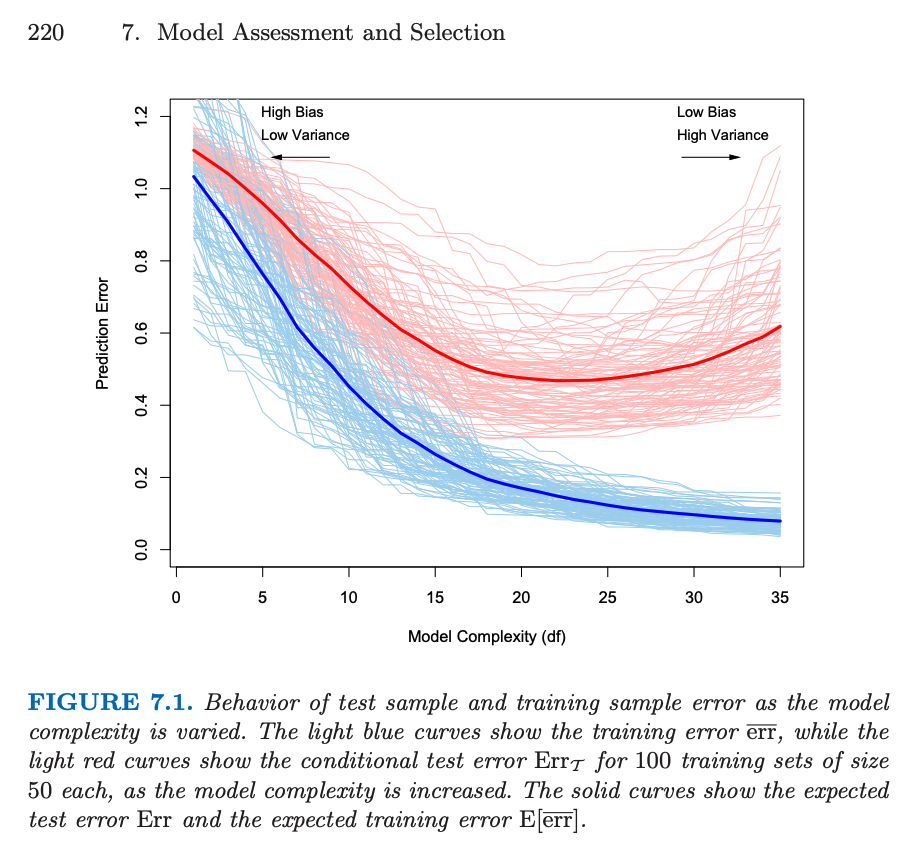
\includegraphics{ELSfig71.png}

\end{frame}

\begin{frame}

\begin{block}{Conclusion}

(from Figure 7.1)

The training error \(\overline{\text{err}}\) is not a good estimate for
the \(\text{Err}_{\cal T}\) nor the \(\text{Err}\).

If we are in a \emph{data rich situation} we ``just'' divide our data
into three parts, and use

\begin{itemize}
\tightlist
\item
  one for training
\item
  one for validation (model selection)
\item
  one for testing (model assessment)
\end{itemize}

A typical split might be 50-60\% training and 20-25\% validation and
test, but this depends on the complexity of the model to be fitted and
the signal-to-noise ratio in the data.

The focus in Ch 7 of ELS is to present methods to be used in the
situations where we \emph{don´t have enough data} to rely on the
training-validation-testing split.

\end{block}

\end{frame}

\begin{frame}

\begin{block}{Loss function and training error for classification}

\begin{itemize}
\tightlist
\item
  \(X \in \Re^p\)
\item
  \(G \in {\cal G}=\{1,\ldots,K\}\)
\item
  \(\hat{G}(X) \in {\cal G}=\{1,\ldots,K\}\)
\end{itemize}

0-1 loss with \(\hat{G}(X)=\text{argmax}_k \hat{p}_k(X)\)
\[L(G,\hat{G}(X))=I(G\neq \hat{G}(X))\] \(-2\)-loglikelihood loss (why
\(-2\)?): \[ L(G,\hat{p}(X))=-2 \text{log} \hat{p}_G(X)\]

\end{block}

\end{frame}

\begin{frame}

Test error (only replace \(\hat{f}\) with \(\hat{G}\)):
\[ \text{Err}_{\cal T}=\text{E}[L(Y,\hat{G}(X))\mid {\cal T}]\]
\[ \text{Err}=\text{E}[L(Y,\hat{G}(X))\mid {\cal T}]=\text{E} [\text{Err}_{\cal T}]\]

Training error (for 0-1 loss)
\[\overline{\text{err}}=\frac{1}{N}\sum_{i=1}^N I(g_i\neq \hat{g}(x_i))\]
Training error (for \(-2\)loglikelihood loss)
\[\overline{\text{err}}=-\frac{2}{N}\sum_{i=1}^N \text{log}\hat{p}_{g_i}(x_i)\]

\end{frame}

\begin{frame}

\begin{block}{Optimism of the training error rate}

(again - focus is on regression)

First, nothing new, but new notation \((X^0,Y^0)\) to specify that a new
test observation is drawn from the joint distribution \(F\) (both over
new \(X\) and new \(Y\)):

\[\text{Err}_{\cal T}=\text{E}_{X^0,Y^0}[L(Y^0,\hat{f}(X^0))\mid {\cal T}]\]

and then the averaging over the training set (both \(X\)s and \(Y\)s in
the training set):
\[\text{Err}=\text{E}_{\cal T} \text{E}_{X^0,Y^0}[L(Y^0,\hat{f}(X^0))\mid {\cal T}]\]

This is also called \emph{extra-sample error} (in contrast to what we
now will define to be in-sample).

\end{block}

\end{frame}

\begin{frame}

We saw before - from the ELS Figure 7.1, the training error
\(\overline{\text{err}}\) is (in general) less than (or equal to) the
true test error, so not a good estimator for the test error.

\[\overline{\text{err}}=\frac{1}{N} \sum_{i=1}^N L(y_i,\hat{f}(x_i))\]

{[}In Exercise 2.9 we prove that the expected training error is smaller
or equal the expected error of a testset - for MLR. Important to work on
this exercise!{]}

Part of this is due to where the \(X\) values are ``placed''. The test
input vectors need not be ``in the same positions'' as in the training
\(X\) values (when the mean is taken over the full distribution of
\(X\)).

To eliminate this ``confusing fact'', calculations can be made be
assuming the \(X\)-values in the training data are kept fixed - and this
is called the \emph{in-sample error}. (We did the same in TMA4267 using
the Fahrmeir et al book, Chapter 3.4.)

\end{frame}

\begin{frame}

\begin{block}{In-sample error}

\[\text{Err}_{\text{in}}=\frac{1}{N}\sum_{i=1}^N \text{E}_{Y^0}[L(Y_i^0,\hat{f}(x_i))\mid {\cal T}]\]

Observe that we now take the expected value over distribution of the
response - but that the (new) responses are found at the original
training points. The training predictor positions \(x_i\),
\(i=1,\ldots, N\) are fixed. In addition the responses in the training
data are also kept fixed, so the only random quantity here is the new
responses at the fixed predictors.

\end{block}

\end{frame}

\begin{frame}

\begin{block}{Optimism}

is defined as the difference between the in-sample error and the
training error:

\[ \text{op}=\text{Err}_{\text{in}}-\overline{\text{err}}\]

\end{block}

\begin{block}{Average optimism}

is defined as the expected value of the optimism, where the expectation
is taken over the distribution of the training responses - denoted
\({\bf y}\) (training predictors still kept fixed):

\[ \omega=\text{E}_{\bf y}(op)=\text{E}_{\bf y}(\text{Err}_{\text{in}})-\text{E}_{\bf y}(\overline{\text{err}})\]

Observe that if we write \({\cal T}\) then the expectation is taken over
the distribution of both the predictors and responses in the training
set, and we here write \({\bf y}\) for taking the distribution only over
the reponses in the training set (not the predictors in the training
set).

So: we will focus on ``modelling'' \(\omega\), ``instead of''
\(\text{Err}\).

\end{block}

\end{frame}

\begin{frame}

\begin{block}{Covariance result}

For squared error (see ELS exercise 7.4), 0-1 loss, and ``other loss
functions'' it can be shown

\[ \omega=\frac{2}{N} \sum_{i=1}^N \text{Cov}(\hat{y}_i,y_i)\]
Interpretation:

\begin{itemize}
\tightlist
\item
  how much the training error \emph{underestimates} the true error
  depends on how strongly the observed response \(y_i\) affects its own
  prediction \(\hat{y}_i\).
\item
  the \emph{harder} we fit the data the greater the covariance - which
  increases the expected (averaged) optimism.
\end{itemize}

\end{block}

\end{frame}

\begin{frame}

\begin{block}{Expected in-sample prediction error}

\[ \text{E}_{\bf y}(\text{Err}_{\text{in}})=\text{E}_{\bf y}(\overline{\text{err}})+\frac{2}{N} \sum_{i=1}^N \text{Cov}(\hat{y}_i,y_i)\]
This is the starting point for several methods to ``penalize'' fitting
complex models!

\end{block}

\end{frame}

\begin{frame}

\begin{block}{Result for \(\omega\)}

Additive error model and squared loss: \(Y=f(X)+\varepsilon\), with
\(\hat{y}_i\) obtained by a linear fit with \(d\) inputs (or basis
functions) \[\omega=2 \frac{d}{N}\sigma_{\varepsilon}^2\]

Proof? We look at a generalization in ELS exercise 7.5.

Observe that the optimism increases with \(d\) and decreases with \(N\).

Comment: versions of the formula hold approximately for other error
models than linear with squared loss (ELS mention binary data and
entropy loss), but not in general for 0-1 loss (page 231, bottom, with
reference to Efron 1986 - consult the ELS book).

\end{block}

\end{frame}

\begin{frame}

\begin{block}{Three ways to perform model selection}

\begin{itemize}
\item
  Estimate of expected in-sample prediction error (ELS Ch 7.5-7.6): We
  may develop the average optimism for a class of models that are linear
  in the parameters (Mallows Cp, AIC, BIC, \ldots) - and compare models
  of different complexity using
  \(\text{E}_{\bf y}(\text{Err}_{\text{in}})\). Remark: in-sample error
  is not of interest, but used to choose between models effectively.
\item
  Estimate \(\text{Err}\) (ELS Ch 7.10-7.11): We may instead use
  resampling methods (cross-validation and bootstrapping) to estimate
  \(\text{Err}\) directly (and use that for model selection and
  assessment).
\item
  In the data rich approach: we have so much data that we use a separate
  validation set for model selection (and a separate test set for model
  assessment). That is not the focus of ELS Ch 7.
\end{itemize}

\end{block}

\end{frame}

\begin{frame}

\begin{block}{Estimates of (expected) in-sample prediction error}

We have the following result:

\[ \text{E}_{\bf y}(\text{Err}_{\text{in}})=\text{E}_{\bf y}(\overline{\text{err}})+\frac{2}{N} \sum_{i=1}^N \text{Cov}(\hat{y}_i,y_i)\]
where now \[ \omega=\frac{2}{N} \sum_{i=1}^N \text{Cov}(\hat{y}_i,y_i)\]
We now want to get an estimate of the average optimism, to get an
estimate of the in-sample prediction error:

\[ \widehat{\text{Err}_{\text{in}}}=\overline{\text{err}}+\hat{\omega}\]

Comment: observe that \(\overline{\text{err}}\) is now an estimate of
\(\text{E}_{\bf y}(\overline{\text{err}})\) and even though we write
\(\widehat{\text{Err}_{\text{in}}}\) we are aiming to estimate
\(\text{E}_{\bf y}(\text{Err}_{\text{in}})\). Focus now is on
\(\hat{\omega}\)!

\end{block}

\end{frame}

\begin{frame}

\begin{block}{\(C_p\) statistics}

for squared error loss (follows directly from the \(\omega\)-result for
additive error model)

\[C_p=\overline{\text{err}}+2\frac{d}{N}\hat{\sigma}_{\varepsilon}^2\]
where \(\hat{\sigma}_{\varepsilon}^2\) is estimated from a ``low-bias
model'' (in MLR we use a ``full model'').

(This method is presented both in TMA4267 and TMA4268, see also exam
question
\href{https://www.math.ntnu.no/emner/TMA4267/2017v/Exam/eV2015.pdf}{Problem
3 in TMA4267 in 2015} and
\href{https://www.math.ntnu.no/emner/TMA4267/2017v/Exam/lV2015.pdf}{solutions}.)

\end{block}

\end{frame}

\begin{frame}

\begin{block}{Akaike information criterion (AIC)}

Based on different asymptotic (\(N \rightarrow \infty\)) relationship
for log-likelihood loss functions

\[ -2 \text{E}[\log P_{\hat{\theta}}(Y)]\approx - \frac{2}{N} \text{E}[\text{loglik}]+2 \frac{d}{N} \]

\begin{itemize}
\tightlist
\item
  \(P_{\hat{\theta}}(Y)]\): family of density for \(Y\) where the true
  density is included
\item
  \(\hat{\theta}\): MLE of \(\theta\)
\item
  \(\text{loglik}]\): maximized log-likelihood
  \(\sum_{i=1}^N \log P_{\hat{\theta}}(y_i)\)
\end{itemize}

\end{block}

\end{frame}

\begin{frame}

\textbf{Logistic regression with binomial loglikelihood}

\[ \text{AIC}=- \frac{2}{N} \text{loglik}+2 \frac{d}{N}\]
\textbf{Multiple linear regression} if variance
\(\sigma_{\varepsilon}^2=\hat{\sigma}_{\varepsilon}^2\) assumed known
then AIC is equivalent to \(C_p\).

For nonlinear or similar models then \(d\) is replaced by some measure
of model complexity.

\end{frame}

\begin{frame}

\textbf{AIC as function of tuning parameter} (back to squared error
loss)

We have a set of models \(f_{\alpha}(x)\) indexed by some tuning
parameter \(\alpha\).

\[\text{AIC}(\alpha)=\overline{\text{err}}(\alpha)+2 \frac{d(\alpha)}{N}\hat{\sigma}_{\varepsilon}^2\]

\begin{itemize}
\tightlist
\item
  \(\overline{\text{err}}(\alpha)\): training error
\item
  \(d(\alpha)\) number of parameters
\item
  \(\hat{\sigma}_{\varepsilon}^2\) estimated variance of large model
\end{itemize}

The model complexity \(\alpha\) is chosen to minimize
\(\text{AIC}(\alpha)\).

This is not true if the models are chosen adaptively (for example basis
functions) this formula underestimates the optimism - and we may regard
this as the \emph{effective number of parameters} is larger than \(d\).

\end{frame}

\begin{frame}

\begin{block}{The effective number of parameters}

The number of parameters \(d\) can be generalized into an
\emph{effective number of parameters}. We will look at linear fitting
method:

\[ \hat{\bf y}={\bf Sy}\] where \({\bf S}\) as a \(n \times n\) matrix
depending on covariates \(x_i\) but not responses \(y_i\).

\begin{itemize}
\tightlist
\item
  MLR \({\bf H}={\bf X}({\bf X}^T{\bf X})^{-1}{\bf X}^T\)
\item
  cubic smoothing splines
\item
  ridge regression
\end{itemize}

The effective number of parameters is

\[\text{df}({\bf S})=\text{trace}({\bf S})\] Remember that the trace of
a square matrix is the sum of the diagonal elements, and trace is often
denoted tr.

\end{block}

\end{frame}

\begin{frame}

What is the trace (tr) for MLR?

\(\text{tr}({\bf H})=\text{tr}({\bf X}({\bf X}^T{\bf X})^{-1}{\bf X}^T)=\text{tr}(({\bf X}^T{\bf X})^{-1}{\bf X}^T{\bf X})=\text{tr}({\bf I})_{p+1}=(p+1)\)
if intercept model with \(p\) covariates.

\end{frame}

\begin{frame}

\textbf{Additive error model and squared loss:} \(Y=f(X)+\varepsilon\)
with \(\text{Var}(\varepsilon)=\sigma_{\varepsilon}^2\) then
\[ \sum_{i=1}^N \text{Cov}(\hat{y}_i,y_i)=\text{trace}({\bf S})\sigma_{\varepsilon}^2\]
leading to a generalization
\[\text{df}(\hat{{\bf y}})=\frac{\sum_{i=1}^N \text{Cov}(\hat{y}_i,y_i)}{\sigma_{\varepsilon}^2}\]
See exercise 7.5 to prove this.

We return to this formula when we look at neural networks with quadratic
penalization (weigth decay, ridge regularization) in Part 3.

\end{frame}

\begin{frame}

\begin{block}{Cross-validation (CV)}

(ELS Ch 7.10, 7.12 - most should be known from TMA4268)

The aim is to estimate \(\text{Err}_{\cal T}\), but from simulation
analyses (ELS Ch 7.12) it turns out that cross-validation estimates
\(\text{Err}\) ``the best''.

The starting point for the method is that we only have one training set
- and try to use that for either model selection or model assessment
(not both).

What to do when both is needed, is not covered in this chapter. Nested
cross-validations aka two-layers of cross-validation is one possibility.
Another is to set aside data for a test set for model assessment, but
use the training set in cross-validation for model selection.

\end{block}

\end{frame}

\begin{frame}

\begin{block}{Formal set-up for model assessment}

The allocation of observation \(\{1,\ldots,N\}\) to folds
\(\{1,\ldots,K\}\) is done using an indexing function
\(\kappa: \{1,\ldots,N\} \rightarrow \{1,\ldots,K\}\), that for each
observation allocate the observation to one of \(K\) folds.

Further, \(\hat{f}^{-k}(x)\) is the fitted function, computed on the
observations except the \(k\)th fold (the observations from the \(k\)th
fold is removed).

The CV estimate of the expected prediction error
\(\text{Err}=\text{Err}=\text{E}_{\cal T} \text{E}_{X^0,Y^0}[L(Y^0,\hat{f}(X^0))\mid {\cal T}]\)
is then
\[ \text{CV}(\hat{f})=\frac{1}{N}\sum_{i=1}^N L(y_i,\hat{f}^{-k(i)}(x_i))\]

\end{block}

\end{frame}

\begin{frame}

\begin{block}{Formal set-up for model selection}

The indexing function \(\kappa\) is unchanged, and for the fitting
function we add a tuning parameter \(\alpha\): \(f(x,\alpha)\) such that
\(\hat{f}^{-k}(x,\alpha)\) is the fitted function using tuning parameter
\(\alpha\), with the \(k\)th fold removed from the model fitting.

The expected prediction error is estimated by

\[ \text{CV}(\hat{f},\alpha)=\frac{1}{N}\sum_{i=1}^N L(y_i,\hat{f}^{-k(i)}(x_i,\alpha))\]

We find the best tuning parameter \(\hat{\alpha}\) that minimize the
\(\text{CV}(\hat{f},\alpha)\). Alternatively the \emph{one-standard
error rule} can be used: choose the most parsimonious (``smallest'')
model whose error is no more than one standard error above the error of
the best model.

This best chosen model is then fit to all the data. (ELS page 242).

\end{block}

\end{frame}

\begin{frame}

\begin{block}{Choice of \(K\)}

\begin{itemize}
\tightlist
\item
  Popular choices are 5 and 10 based on observations in simulation
  studies- and arguments similar to a bias-variance trace off (\(K=1\)
  has lowes bias)
\item
  \(K=N\) is called \emph{leave-one-out} cross-validation LOOCV, and
  gives the lowest bias for estimating the \(\text{Err}\).
\end{itemize}

\end{block}

\end{frame}

\begin{frame}

\begin{block}{Generalized cross-validation (GCV)}

For LOOCV with squared loss and linear fitting. Remember
\[ \hat{\bf y}={\bf Sy}\] For many fitting methods (including MLR)

\[ \frac{1}{N}\sum_{i=1}^N [y_i-\hat{f}^{-i}(x_i)]^2=\frac{1}{N}\sum_{i=1}^N [\frac{y_i-\hat{f}(x_i)}{1-S_{ii}}]^2\]
where \(S_{ii}\) is the \(i\)th diagonal element of \({\bf S}\). This
leads to the GCV approximation:

\[ \text{GCV}(\hat{f})=\frac{1}{N}\sum_{i=1}^N [\frac{y_i-\hat{f}(x_i)}{1-\text{tr}({\bf S})/N}]^2\]
where we recognise the effective number of parameters
\(\text{trace}({\bf S})\). In some settings the
\(\text{trace}({\bf S})\) is computed more easily than the individual
elements \(S_{ii}\).

\end{block}

\end{frame}

\begin{frame}

\begin{block}{The wrong and the right way to do cross-validation}

In short: make sure that all part of the model fit process is ``inside''
the CV.

See learning material from TMA4268:
\href{https://www.math.ntnu.no/emner/TMA4268/2019v/5Resample/5Resample.html\#the_right_and_the_wrong_way_to_do_cross-validation}{Module
5: Resampling}, and I also recommend to work on
\href{https://www.math.ntnu.no/emner/TMA4268/2019v/5Resample/5Resample.html\#problem_3:_selection_bias_and_the_\%E2\%80\%9Cwrong_way_to_do_cv\%E2\%80\%9D}{Problem
3} with \href{}{solutions}

\end{block}

\end{frame}

\begin{frame}

\begin{block}{Bootstrap methods}

(ELS Ch 7.11 - bootstrapping is known from TMA4268 and TMA4300, but not
the special case of estimating \(\text{Err}\)).
\href{https://www.math.ntnu.no/emner/TMA4268/2019v/5Resample/5Resample.html\#the_bootstrap}{Bootstrap
in TMA4268}

\textbf{Notation:} \({\bf Z}=(z_1,\ldots,z_N)\) is the training set with
\(z_i=(x_i,y_i)\).

\textbf{Aim:} Of interest is some quantity calculated from the data
\({\bf Z}\), denoted \(S({\bf Z})\). We will have focus on the expected
prediction error.

\textbf{Resampling:} We draw with replacement from \({\bf Z}\) a total
of \(N\) observastions into \({\bf Z}^{*b}\). We repeat this \(B\)
times.

\textbf{Estimator for expected predicted error \(\text{Err}\):}

\[\widehat{\text{Err}}_{\text{boot}}=\frac{1}{B}\frac{1}{N}\sum_{b=1}^B \sum_{i=1}^N L(y_i,\hat{f}^{*b}(x_i))\]

\end{block}

\end{frame}

\begin{frame}

However - \(\widehat{\text{Err}}_{\text{boot}}\) is not a good
estimator: bootstrap datasets are acting as training data and the
original data as a test sample - and the two samples have observations
in common.

This overlap can make predictions too good. Remeber, in CV we have no
overlap.

\textbf{Q:} What is the probability that observation \(i\) is included
in bootstrap sample \(b\)?

\end{frame}

\begin{frame}

The problem is given in TMA4268 Module 5 as
\href{https://www.math.ntnu.no/emner/TMA4268/2019v/5Resample/5Resample.html\#recexboot}{Problem
1} with (handwritten)
\href{https://www.math.ntnu.no/emner/TMA4268/2019v/5Resample/5Resample-sol.pdf}{solutions}.

The answer is \(1-(1-\frac{1}{N})^N\approx 1-e^{-1}=0.632\).

Why is this relevant?

What if we try to change the bootstrap \(\text{Err}\) estimator - so
that we for each observation \(i\) only keep predictions from bootstrap
samples this observation is not present? Then we would mimick the
CV-estimator.

\end{frame}

\begin{frame}

The \emph{leave-one-out} bootstrap estimate:

\[\widehat{\text{Err}}^{(1)}=\frac{1}{N} \sum_{i=1}^N \frac{1}{\lvert C^{-i} \rvert} \sum_{b \in C^{-i}} L(y_i,\hat{f}^{*b}(x_i))\]
where \(C^{-i}\) are the indices in the bootstrap sample \(b\) that do
not contain observation \(i\), and \(\lvert C^{-i} \rvert\) is the
number of samples. (\(B\) must be large enough that we do not get any
\(C^{-i}\)s that are empty, or leave out these zero sete in the
formula.)

Comment: this is also called out-of-bootstrap, and is closely connected
to the popular out-of-bag estimate for random forests.

\end{frame}

\begin{frame}

There is an addition fix to make the estimate even better.

Since the average number of distinct observations in each bootstrap
sample is approximately \(0.632 N\) - and the bootstrap sample behaves
like a traning set - this gives a socalled traning-set-size bias
(similar to C with \(K=2\)), meaning that the leave-one-out bootstrap
estimator will be \emph{biased upwards}. This can be fixed by weighing
together the leave-one-out boostrap estimator with the training error.

The ``.632'' estimator:

\[\widehat{\text{Err}}^{(.632)}=0.368 \overline{\text{err}}+0.632 \widehat{\text{Err}}^{(1)}\]

According to ELS (page 251): the derivation of the .632 estimator is
complex, and the estimator is expected to work well in situation where
the data is not overfitted, but may break down in overfit situations.

According to CASI (page 323) the .632 rule is less variable than the
leave-one-out CV.

Example of this on page 251-252: two equal size classes where predictors
independent of class, classification with \(1\)NN gives
\(\overline{\text{err}}=0\), \(\widehat{\text{Err}}^{(1)}=0.5\) and thus
\(\widehat{\text{Err}}^{(.632)}=0.632\cdot 0.5=0.316\), where here the
true error rate is \(0.5\).

\end{frame}

\begin{frame}

There is an improved version of the estimator - taking into account the
amount of overfitting, leading to an adjustment to the weight
\(w=0.632\) (and \(1-w=0.368\)) dependent on a socalled
\emph{no-information error rate}=\(\gamma\)=the error rate of the
prediction rule when predictors and class labels are independent.

\[\hat{\gamma}=\frac{1}{N^2}\sum_{i=1}^{N}\sum_{i´=1}^N L(y_i,\hat{f}(x_{i´}))\]
Further the \emph{relative overfitting rate} is defined to be

\begin{block}{\[ \hat{R}=\frac{\widehat{\text{Err}}^{(1)}-\overline{\text{err}}}{\hat{\gamma}-\overline{\text{err}}}\]}

Finally, the ``.632+''-estimator is

\[\widehat{\text{Err}}^{(.632+)}=(1-\hat{w}) \overline{\text{err}}+ \hat{w} \widehat{\text{Err}}^{(1)}\]
where \(\hat{w}=\frac{0.632}{1-0.368 \hat{R}}\).

For details on this approach consult ELS page 252-253.

\end{block}

\end{frame}

\begin{frame}{Conclusions: Model selection and assessment}
\protect\hypertarget{conclusions-model-selection-and-assessment}{}

\begin{itemize}
\tightlist
\item
  in a perfect world we would be rich on data and can divide available
  data into sets for training, validation and testing
\item
  cool covariance-result on expected optimism for training error related
  to in-sample prediction error (the covariance) - that is used for
  finding model selection criteria (but not for model assessment)
\item
  estimating expected prediction (test) error for a particular training
  set is not easy in general (if we only have this one training set),
  but cross-validation and bootstrapping may provide reasonable
  estimates of the expected test error \(\text{Err}\).
\end{itemize}

\end{frame}

\begin{frame}{Exercises}
\protect\hypertarget{exercises}{}

The exercises are from the ELS book, Chapters 2 and 7. Solutions to the
exercises will be posted, see also under References for solutions posted
by different authors.

\begin{block}{Curse of dimensionality}

Read pages 22-23 and then answer Exercise 2.3 - which is to ``Derive
equation (2.24).''

Important take home messages:

\begin{itemize}
\tightlist
\item
  All sample points are close to an edge of the sample.
\item
  If data are uniformly distributed in an hypercube in \(p\) dimensions,
  we need to cover \(r^{1/p}\) of the the range of each input variable
  to capture a fraction \(r\) of the observations.
\end{itemize}

\end{block}

\begin{block}{Expected training and test MSE for linear regression}

Exercise 2.9.

Important take home message: We have proven (for MLR) that the expected
test MSE is always at least as large as the expected training MSE.

\end{block}

\end{frame}

\begin{frame}

\begin{block}{Look into the derivation for the bias and variance}

(no solutions posted)

for \(k\)NN in Equation 7.10 and OLS in Equation 7.11 on pages 222-223.

\end{block}

\begin{block}{Establish the average optimism in the training error}

Exercise 7.4

\end{block}

\begin{block}{Relate the covariance to the trace of a linear smoother}

Exercise 7.5

\end{block}

\begin{block}{Perform best subset linear regression and compute
different error rates}

Exercise 7.9

\end{block}

\end{frame}

\begin{frame}{Solutions to exercises}
\protect\hypertarget{solutions-to-exercises}{}

Please try yourself first, or take a small peek - and try some more -
before fully reading the solutions. Report errors or improvements to
\href{mailto:Mette.Langaas@ntnu.no}{\nolinkurl{Mette.Langaas@ntnu.no}}.
(The solutions given here are very similar to the UiO solutions, see
link under References.)

(under construction, to be linked in)

\begin{itemize}
\tightlist
\item
  2.3, 2.9, 7.4, 7.5
\item
  7.9
\end{itemize}

\end{frame}

\begin{frame}{References}
\protect\hypertarget{references}{}

\begin{itemize}
\item
  \href{https://waxworksmath.com/Authors/G_M/Hastie/hastie.html}{ELS
  solutions to exercises}
\item
  ELS solutions from UiO
  \url{https://www.uio.no/studier/emner/matnat/math/STK-IN4300/h20/exercises.html}
\item
  ELS official errata:
  \url{https://web.stanford.edu/~hastie/ElemStatLearn/errata2.html}
\item
  R Markdown Cookbook:
  \url{https://bookdown.org/yihui/rmarkdown-cookbook/}
\item
  R Markdown cheat sheet:
  \textgreater{}\url{https://rstudio.com/wp-content/uploads/2015/03/rmarkdown-reference.pdf}\textgreater{}
\item
  \url{https://en.wikipedia.org/wiki/Camel_case}
\item
  \url{https://en.wikipedia.org/wiki/Snake_case}
\item
  (CASI) Computer Age Statistical Inference, Efron and Hastie (2017)
  Chapter 12: Cross-Valiation and \(C_p\) Estimates of Prediction Error.
  \url{https://web.stanford.edu/~hastie/CASI_files/PDF/casi.pdf}
\item
  Burnham and ANdersen (2002): Model Selection and Multimodel Inference:
  A Practical Information-Theoretic Approach. Springer. Chapter 7:
  Statistical Theory and Numerical Results
  \url{https://link.springer.com/chapter/10.1007/978-0-387-22456-5_7}
\end{itemize}

\end{frame}

\end{document}
